\documentclass{article}
\usepackage[utf8]{inputenc}
\usepackage[utf8]{inputenc}

\usepackage{amssymb}
\usepackage{amsfonts}
\usepackage{amsmath}
\usepackage{amsthm}
\usepackage{microtype}
\usepackage{physics}
\usepackage{bbm}

\usepackage{hyperref}
\usepackage{enumitem}
\usepackage{nicematrix}
\usepackage{mathtools}

\usepackage{amsmath}
\usepackage{algorithm,algpseudocode,float}
\usepackage{graphicx}
\usepackage{caption}
\usepackage{subcaption}
\usepackage{xcolor}

\DeclareMathOperator{\EX}{\mathbb{E}} % expected value

\makeatletter
\def\BState{\State\hskip-\ALG@thistlm}
\makeatother

\title{Project Report\\Stock Price Prediction using Sentiment Analysis\\ MPCS 53113: Natural Language Processing}
\author{Shobhit Verma, Ashish Verma \\ \texttt{shobhitv@uchicago.edu, ashishv@uchicago.edu}}

\begin{document}

\maketitle

\section{Abstract}
Prediction of the stock prices has been an age old problem. Theoretically, the stock price of a company is dependant on a variety of factors, as per [1]. Thanks to the large number of social media channels and news feeds online, we have access to information on some of these factors (example, employee layovers, takeovers and mergers, etc). In this project, we aim to capture and quantify this information for a specific time period and correlate it with the change in stock price in said time period. Because of how most stock exchanges function, a time period is defined as a day. 

There are many ways to approach this - we could take a macroeconomic approach and correlate the stock price index (tracking stock price of a number of companies) with information from macroeconomic news feeds, or we could take a microeconomic approach wherein we focus on a specific company (say, google) and fetch news articles and tweets specific to that company only. We utilize a dataset of 25 companies, each of which belongs to the S\&P500 index. 

Using machine learning for stock price prediction is not new - Ravikumar et al. [2] demonstrated that some viable results may be achieved by using features derived from historical price data as inputs to ML models to predict movement (classification, up or down) and delta in stock price (regression, a real valued number). We use this work and extend it by trying to use a new feature - ratio of positive tweets to total tweets about that company on that day.

We try to demonstrate that adding new features based on sentiment can serve to improve the task of prediction, using the same models in [2]. The first part of the project is building the sentiment classifier. For this, we use the sentiment140 dataset (annotated collection of 1.6M tweets) to train models - RNNs, LSTMs and GRUs. Then, we required to evaluate the performance of this classifier on a dataset of financial tweets. Using [3], we fetched about 1M financial tweets on 25 S\&P500 companies that were unannotated, and about 5000 tweets that are annotated with sentiment. Using the latter to justify performance of our sentiment classifier, we annotate the former with sentiment. Then, extracting the number of positive and negatove tweets per company per day is another task - from which we extract company specific positive tweets ratio per day.
This brings us to the second part of our project - using classifiers to predict simply whether the stock price goes up or down (predicting momentum) and using regressors to predict the change in stock price in a particular day. (difference in closing price and opening price). We use SVMs, Logistic Regression, k Nearest Neighbours for the classification task. For the regression task, we use SVRs and Linear Regression.

\section{Introduction}
According to Wikipedia, a stock market, equity market, or share market is the aggregation of buyers and sellers of stocks (also called shares), which represent ownership claims on businesses. Investopedia says that the share price is determined by ‘demand and supply’ of the shares in the market. Typically, shares with higher demand have higher prices and shares with higher supply have lower prices. Stock market brokers try to be good at their jobs by being present physically at the stock exchanges, and trying to measure public sentiment before making a decision (buy/sell). In today's digital world, every opinion is shared on twitter in intervals of just a few seconds. According to [4], about 300,000 tweets are made per minute. While it is challenging to skim, clean and find relevant information from raw tweet data, there is no denying that some important information is encoded here that can help us in automating certain decision processes.

\section{Related work}
[5] is a similar project that attempts to solve the same problem of stock price prediction using Tweets. It uses pre-trained Glove and Sentiment-Specific Word Embeddings and NLTK tokenizer, and then predicts a positive or negative sentiment for a particular tweet using a softmax classifier. Using this positive or negative sentiment, a prediction is made if the stock price will increase, or decrease. We extend this work by exploring more models for sentiment classification. Further, we not only predict momentum in a classification task, but also try to predict the absolute delta in the stock price as a regression task.

[2] explores the use of multiple historical stock price datasets of organizations from S\&P500 index, and using them together to train regression models (linear, SVM, Decision Trees, Random Forest). It also introduces the concepts of derived attributes such as Momentum, Volatility, and Average Volatility and explains how they help in regression tasks, which we take inspiration from in our project. 

\section{Detailed description of our work}
Our pipeline looks as follows. For now, assume day $d_1$ and day $d_N$ are some predetermined dates.
\begin{enumerate}
    \item Using a dataset of tweets annotated with positive or negative sentiment, train a binary classification model that classifies a textual tweet into a sentiment - positive or negative.
    \item Evaluate the performance of the sentiment analysis annotator on unseen tweets.
    \item For each of the 25 companies we consider in the S\&P500:
    \begin{enumerate}
        \item Get tweets from day $d_1$ to day $d_N$.
        \item Get historical stock price data from day $d_1$ to day $d_N$, and derive deterministic features (momentum, delta, volatility, average volatility) - populating a table of $N$ entries (one for each day)
        \item Annotate the tweets fetched with positive and negative.
        \item For each day, add the ratio of positive tweets to total tweets, and use this as a new feature, add it to the table of historical price data.
    \end{enumerate}
    \item Now, using the features as Volatility, Average Volatility and positive sentiment ratio, train a classification model for predicting momentum, and a regression model for predicting delta of stock price.
\end{enumerate}

\subsection{Building a sentiment classifier}
We have used 3 models for this task - RNNs, LSTMs and GRUs. We use the sentiment140 dataset - a set of apprx 1.6M tweets annotated with positive (1) or negative (0) class. A drawback is that there are only 2 classes in this dataset, however, it is one of the most widely used datasets for classification tasks. 
We use glove embeddings of words as input to the recurrent networks each stage, and keep the size of the hidden dimension equal to the dimension of the embedding used. Glove provides embeddings of different dimensions - 50, 100 and 300. We take this as a hyperparameter and try to search for the best embedding dimension. Figures 1, 2, and 3 below show how the learning curve varies for dimensions 50 and 100.
Apart from the dimension, we also tried to vary the number of stacked layers, and dropout. Figures 4, 5 show a comparision of the same for RNN and GRU.
\begin{figure*}[ht!]
    \centering
    \begin{subfigure}[t]{0.5\textwidth}
        \centering
        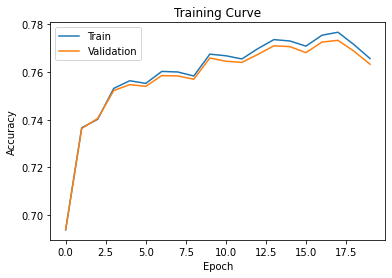
\includegraphics[height=1.5in]{img/sa-dim-search/rnn-training-dim50}
        \caption{Dimension = 50}
    \end{subfigure}%
    ~ 
    \begin{subfigure}[t]{0.5\textwidth}
        \centering
        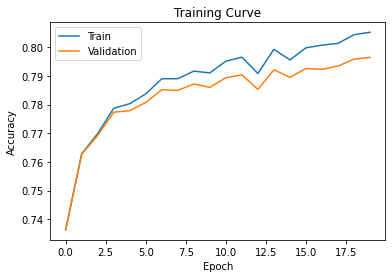
\includegraphics[height=1.5in]{img/sa-dim-search/rnn-training-dim100}
        \caption{Dimension = 100}
    \end{subfigure}
    \caption{RNN learning curve with varying dimension}
\end{figure*}
\begin{figure*}[ht!]
    \centering
    \begin{subfigure}[t]{0.5\textwidth}
        \centering
        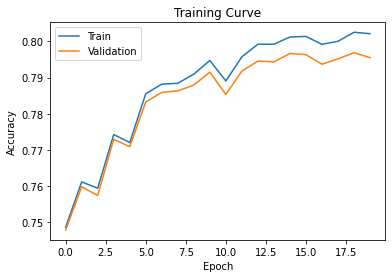
\includegraphics[height=1.5in]{img/sa-dim-search/lstm-training-dim50}
        \caption{Dimension = 50}
    \end{subfigure}%
    ~ 
    \begin{subfigure}[t]{0.5\textwidth}
        \centering
        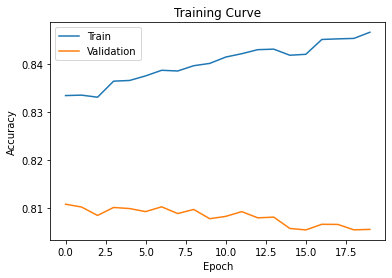
\includegraphics[height=1.5in]{img/sa-dim-search/lstm-training-dim100}
        \caption{Dimension = 100 : increasing training accuracy and falling validation accuracy shows overfitting}
    \end{subfigure}
    \caption{LSTM learning curve with varying dimension}
\end{figure*}
\begin{figure*}[ht!]
    \centering
    \begin{subfigure}[t]{0.5\textwidth}
        \centering
        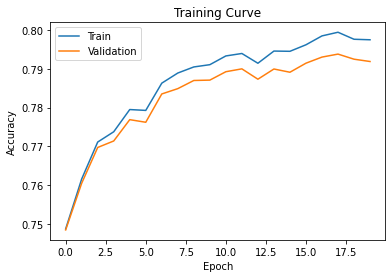
\includegraphics[height=1.5in]{img/sa-dim-search/gru-training-dim50}
        \caption{Dimension = 50}
    \end{subfigure}%
    ~ 
    \begin{subfigure}[t]{0.5\textwidth}
        \centering
        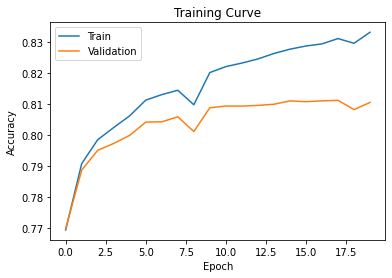
\includegraphics[height=1.5in]{img/sa-dim-search/gru-training-dim100}
        \caption{Dimension = 100}
    \end{subfigure}
    \caption{GRU learning curve with varying dimension}
\end{figure*}
\begin{figure*}[ht!]
    \centering
    \begin{subfigure}[t]{0.5\textwidth}
        \centering
        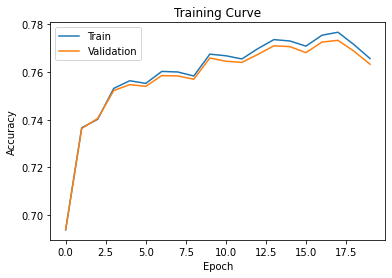
\includegraphics[height=1.5in]{img/sa-dim-search/rnn-training-dim50}
        \caption{stacks = 1}
    \end{subfigure}%
    ~ 
    \begin{subfigure}[t]{0.5\textwidth}
        \centering
        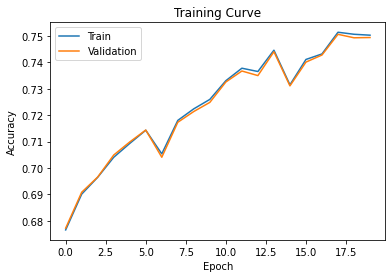
\includegraphics[height=1.5in]{img/sa-dim-search/rnn-training-dim50-stacked-dropout}
        \caption{stacks = 2, dropout = 0.2}
    \end{subfigure}
    \caption{RNN learning curve with varying number of stacks, dropout=0.2}
\end{figure*}
\begin{figure*}[ht!]
    \centering
    \begin{subfigure}[t]{0.5\textwidth}
        \centering
        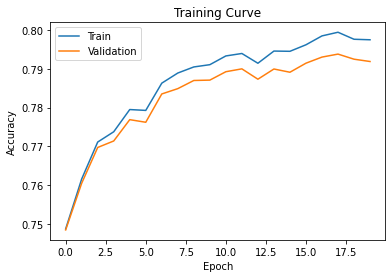
\includegraphics[height=1.5in]{img/sa-dim-search/gru-training-dim50}
        \caption{stacks = 1}
    \end{subfigure}%
    ~ 
    \begin{subfigure}[t]{0.5\textwidth}
        \centering
        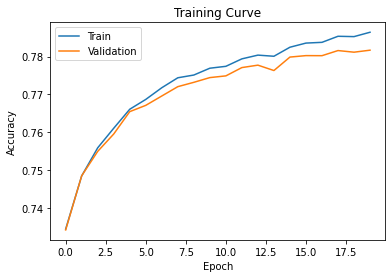
\includegraphics[height=1.5in]{img/sa-dim-search/gru-training-dim50-stacked-dropout}
        \caption{stacks = 2, dropout=0.2}
    \end{subfigure}
    \caption{GRU learning curve with varying number of stacks, dropout=0.2}
\end{figure*}

Increasing the dimension from 50 to 100 and 300 did not lead to any performance gains, and furthermore, in some cases we observe overfitting when going to higher dimensions. Similarly, increasing number of stacks yielded a drop in accuracy scores, and degrading training performance. Hence, we stick with a dimension of 50, and a single (no stacks) recurrent network.

We finally conclude the training subtask by mentioning that all 3 models - RNN, LSTM and GRU - surprisingly yielded a similar preformance in terms of validation accuracy - about 80\%. The last part of this subsection is to use the sentiment analysis classifier to annotate out financial tweets corpus from [3] - about 1M tweets on 25 S\&P companies. This is where there is a bit uncertainty - we can not guarantee annotations will be accurate. However, after annotation, we skimmed the data manually - below are some examples of annotations that suggest a reasonable classification accuracy on this corpus.

\begin{itemize}
    \item @KennyDegu very very little volume. With \$10T you'd think they could have \$SPX  trading at 10,000 by now. - \textcolor{red}{Negative}
    \item Analysts Anticipate Progressive Corp \$PGR to Announce \$1.46 Earnings Per Share - \textcolor{blue}{Positive}
\end{itemize}
Athough not a very reliable metric, we skimmed through many tweets manually and concluded that the sentiment annotation is well enough to at least move forward with the project and conclude our finding in the next subsection.

\subsection{Stock price prediction}
As mentioned earlier, [2] mentions a great way to extract features from historical data. The features used by Ravikumar et al. in [2] are:
\begin{enumerate}
    \item Volatility at day $n$, $V_n$ is defined as $$V_n = (close_{n-1} - close_n)/close_{n-1}$$
    \item Average Volatility - mean of previous five days' volatility.
\end{enumerate}

To this, \textbf{we add a new feature - the ratio of positive tweets about the company to total number of tweets related to the company}, and call this the `sentiment score.'

The targets predicted are:
\begin{enumerate}
    \item Momentum - This is categorical. 1 if stock closes higher than previous day, else 0.
    \item Delta ($d_n$) - This is numerical. $$d_n = close_n - open_n$$
\end{enumerate}

This subsection begins with assuming a well trained sentiment classifier of textual data (from the previous subsection). We start by taking the dataset provided by Bruno et al. [3] - a corpus of apprx. 1M tweets made about 25 S\&P companies. The tweets are dated, between April 9 adn July 16 2020. We annotate this dataset by adding a sentiment column - where the sentiment is the classification made by our sentiment classifier. Now, we require the tweet data specific to each company, which is done as follows - for each comapny in the S\&P500, we create a list of relevant keywords that relate to that company. For example, for the company Merck and Co. (stock ticker \texttt{\$MRK}), the keywords that we search in each tweet for are \texttt{['\$mrk', 'merck', 'pharma', 'pharmaceutical', 'acceleron']}. We then mantain a count of positive and negative tweets by date for this company, and if the tweet contains any of the keyword, we increment the count of the positive/negative tweets for that date. 

We now gather historical stock price data for each company - this is straightforward using the yahoo finance api - for the date range mentioned above. For each day and each company, we have a set of input attributes derived from historical data and  and targets \texttt{(Momentum, Delta)}. We thus have a dataset with the number of labeled data lines as number of companies times the number of days in the date range, and this dataset is used for our classification and regression tasks for stock price prediction.

The analysis of results of this subsection is given in the next section.

\section{Results and analysis}
In each of the two subsections, the input features used are \texttt{(Volatility, AvgVolatility, SentimentScore)}. 

\subsection{Classification - Predicting Momentum}
We used SVMs (with polynomial, rbf, sigmoid and linear kernels), k Nearest Neighbours classifier and Logistic regression. Figures 6 show the validation curves for all the classifiers. The hyperparameter searched for is the regularization parameter.

SVC classifiers with polynomial, RBF and linear kernel returned the best accuracy scores, with accuracy scores of around 98\%. Figure 7 provides the learning curve of all the classifiers.

\begin{figure*}[htb!]
    \centering
    \begin{subfigure}[t]{0.5\textwidth}
        \centering
        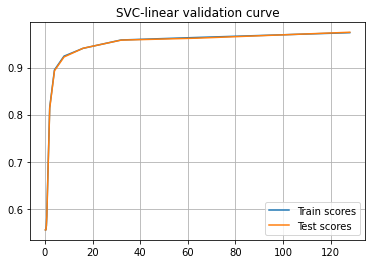
\includegraphics[height=1.5in]{img/momentum-classification/validation-curves/svc-linear}
        \caption{SVC - Linear}
    \end{subfigure}%
    ~ 
    \begin{subfigure}[t]{0.5\textwidth}
        \centering
        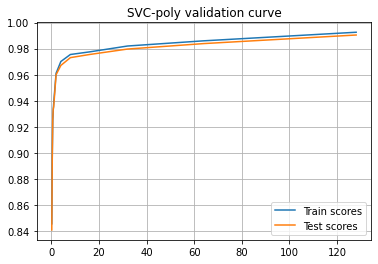
\includegraphics[height=1.5in]{img/momentum-classification/validation-curves/svc-poly}
        \caption{SVC - Poly}
    \end{subfigure}

    \centering
    \begin{subfigure}[t]{0.5\textwidth}
        \centering
        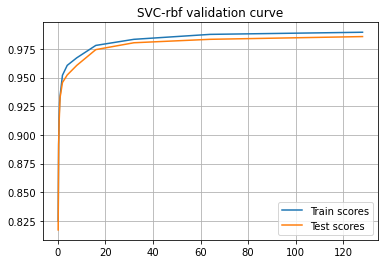
\includegraphics[height=1.5in]{img/momentum-classification/validation-curves/svc-rbf}
        \caption{SVC - RBF}
    \end{subfigure}%
    ~ 
    \begin{subfigure}[t]{0.5\textwidth}
        \centering
        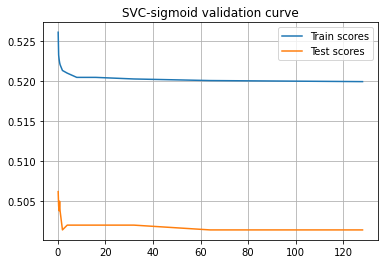
\includegraphics[height=1.5in]{img/momentum-classification/validation-curves/svc-sigmoid}
        \caption{SVC - Sigmoid}
    \end{subfigure}

    \begin{subfigure}[t]{0.5\textwidth}
        \centering
        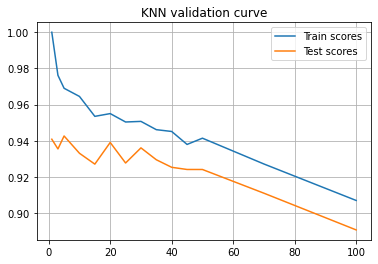
\includegraphics[height=1.5in]{img/momentum-classification/validation-curves/knn}
        \caption{KNN}
    \end{subfigure}%
    ~
    \begin{subfigure}[t]{0.5\textwidth}
        \centering
        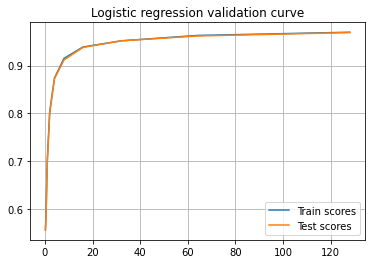
\includegraphics[height=1.5in]{img/momentum-classification/validation-curves/log-regression}
        \caption{Logistic Regression}
    \end{subfigure}

    \caption{Validation curves for classifiers}
\end{figure*}

\begin{figure*}[htb!]
    \centering
    \begin{subfigure}[t]{0.5\textwidth}
        \centering
        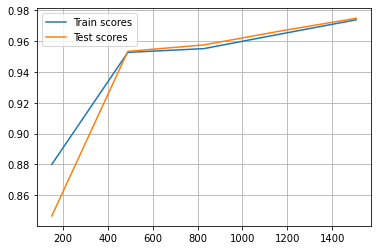
\includegraphics[height=1.5in]{img/momentum-classification/learning-curves/svc-linear}
        \caption{SVC - Linear}
    \end{subfigure}%
    ~ 
    \begin{subfigure}[t]{0.5\textwidth}
        \centering
        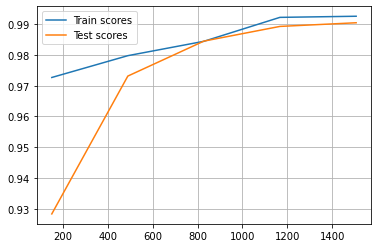
\includegraphics[height=1.5in]{img/momentum-classification/learning-curves/svc-poly}
        \caption{SVC - Poly}
    \end{subfigure}

    \centering
    \begin{subfigure}[t]{0.5\textwidth}
        \centering
        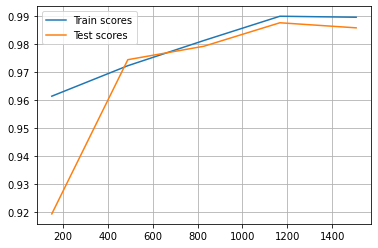
\includegraphics[height=1.5in]{img/momentum-classification/learning-curves/svc-rbf}
        \caption{SVC - RBF}
    \end{subfigure}%
    ~ 
    \begin{subfigure}[t]{0.5\textwidth}
        \centering
        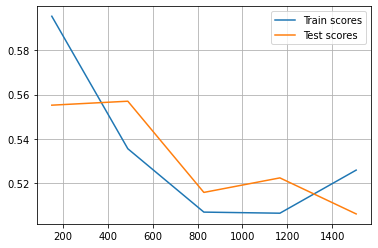
\includegraphics[height=1.5in]{img/momentum-classification/learning-curves/svc-sigmoid}
        \caption{SVC - Sigmoid}
    \end{subfigure}

    \begin{subfigure}[t]{0.5\textwidth}
        \centering
        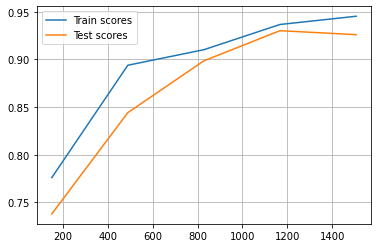
\includegraphics[height=1.5in]{img/momentum-classification/learning-curves/knn}
        \caption{KNN}
    \end{subfigure}%
    ~
    \begin{subfigure}[t]{0.5\textwidth}
        \centering
        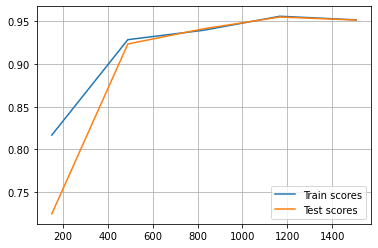
\includegraphics[height=1.5in]{img/momentum-classification/learning-curves/log-regression}
        \caption{Logistic Regression}
    \end{subfigure}

    \caption{Learning curves for classifiers}
\end{figure*}

\clearpage

\subsection{Regression - Predicting Delta}
We used SVMs (with polynomial, rbf, sigmoid and linear kernels) and Linear regression. Figures 8 show the validation curves for all the regression models. The hyperparameter searched for in SVMs the regularization parameter. We use the Men Squared Error as the score for training and validation.

Apart from SVM with sigmoid kernel, all regression models showed a low mean squared error of apprx. $4.7$ on the validation dataset. Figure 9 provides the learning curve of all the regression models.

\begin{figure*}[htb!]
    \centering
    \begin{subfigure}[t]{0.5\textwidth}
        \centering
        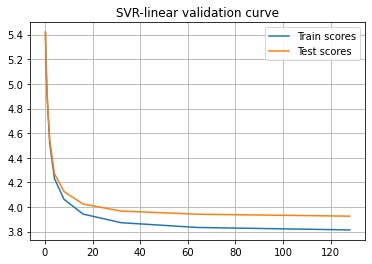
\includegraphics[height=1.5in]{img/delta-regression/validation-curves/svc-linear}
        \caption{SVC - Linear}
    \end{subfigure}%
    ~ 
    \begin{subfigure}[t]{0.5\textwidth}
        \centering
        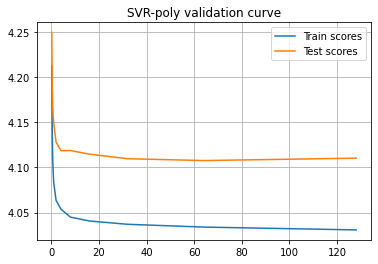
\includegraphics[height=1.5in]{img/delta-regression/validation-curves/svc-poly}
        \caption{SVC - Poly}
    \end{subfigure}

    \centering
    \begin{subfigure}[t]{0.5\textwidth}
        \centering
        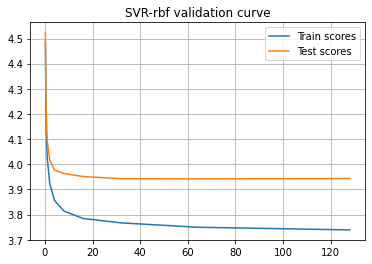
\includegraphics[height=1.5in]{img/delta-regression/validation-curves/svc-rbf}
        \caption{SVC - RBF}
    \end{subfigure}%
    ~ 
    \begin{subfigure}[t]{0.5\textwidth}
        \centering
        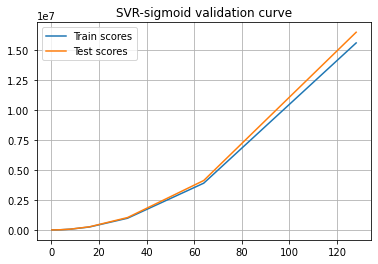
\includegraphics[height=1.5in]{img/delta-regression/validation-curves/svc-sigmoid}
        \caption{SVC - Sigmoid}
    \end{subfigure}

    \caption{Validation curves for classifiers}
\end{figure*}

\begin{figure*}[htb!]
    \centering
    \begin{subfigure}[t]{0.5\textwidth}
        \centering
        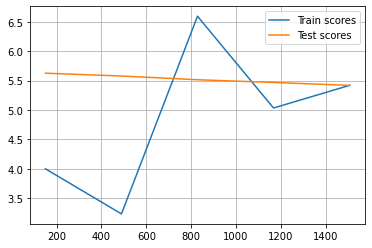
\includegraphics[height=1.5in]{img/delta-regression/learning-curves/svc-linear}
        \caption{SVC - Linear}
    \end{subfigure}%
    ~ 
    \begin{subfigure}[t]{0.5\textwidth}
        \centering
        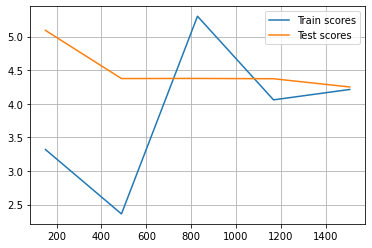
\includegraphics[height=1.5in]{img/delta-regression/learning-curves/svc-poly}
        \caption{SVC - Poly}
    \end{subfigure}

    \centering
    \begin{subfigure}[t]{0.5\textwidth}
        \centering
        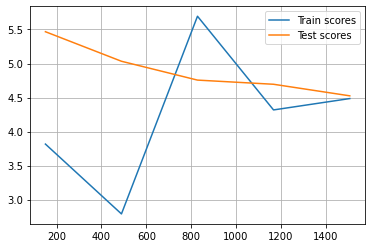
\includegraphics[height=1.5in]{img/delta-regression/learning-curves/svc-rbf}
        \caption{SVC - RBF}
    \end{subfigure}%
    ~ 
    \begin{subfigure}[t]{0.5\textwidth}
        \centering
        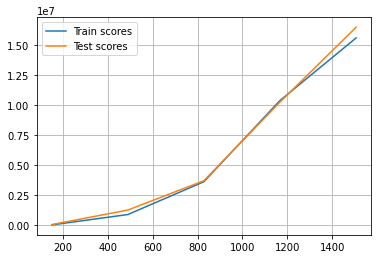
\includegraphics[height=1.5in]{img/delta-regression/learning-curves/svc-sigmoid}
        \caption{SVC - Sigmoid}
    \end{subfigure}

    \begin{subfigure}[t]{0.5\textwidth}
        \centering
        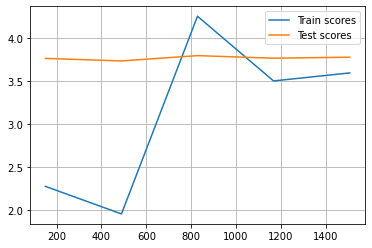
\includegraphics[height=1.5in]{img/delta-regression/learning-curves/lin-reg}
        \caption{Logistic Regression}
    \end{subfigure}

    \caption{Learning curves for classifiers}
\end{figure*}

\clearpage

\pagebreak[4]
\section{Future work}
Realising the limitations of the project, we believe the following improvements could be made to make the predictor more robust.
\begin{enumerate}
    \item Using ensembles to annotate data - currently, we train a bunch of models for sentiment classification. After training, we use the best model, and discard all the others. This results in poor utilisation of trained models. We could instead construct an ensemble of all the performant classifiers and use them to annotate the tweets as positive/negative.
    \item Range of dates of tweets - The size of the dataset of our stock prediction task is linearly dependant on the number of dates we choose our tweets from. While it is easier to fetch historical stock price data, it is much more difficult to fetch tweets spanning over a huge timeline. This demands a high amount of disk storage, compute and memory. However, using disributed computers or sophisticated devices, this may very well be possible.
    \item For cross validation, we only searched the regularisation parameter. However, there are many other parameters that must be searched for obtaining a more performant predictor that generalizes well.
\end{enumerate}

\section{References}

\begin{itemize}
    \item {[1]} \url{https://www.getsmarteraboutmoney.ca/invest/investment-products/stocks/factors-that-can-affect-stock-prices/}
    \item {[2]} S. Ravikumar and P. Saraf, "Prediction of Stock Prices using Machine Learning (Regression, Classification) Algorithms," 2020 International Conference for Emerging Technology (INCET), 2020, pp. 1-5, doi: 10.1109/INCET49848.2020.9154061.
    \item {[3]} Bruno Taborda, Ana de Almeida, José Carlos Dias, Fernando Batista, Ricardo Ribeiro, April 15, 2021, "Stock Market Tweets Data", IEEE Dataport, doi: https://dx.doi.org/10.21227/g8vy-5w61.
    \item {[4]} \url{https://blog.hootsuite.com/twitter-statistics/}
    \item{[5]} \url{https://web.stanford.edu/class/archive/cs/cs224n/cs224n.1174/reports/2743946.pdf}
\end{itemize}


\end{document}